\chapter{Agent-based Modeling and Sensitivity Analysis} \label{ch:literature}

The purpose of this chapter is to briefly introduce the reader to the two main theoretical frameworks of this thesis: Agent-Based Modeling (ABM) and Sensitivity Analysis (SA). In particular, in Sections \ref{abm} and \ref{abm-t}, I present the ABM framework: first, I provide a general overview of Agent-based Modeling; then, I focus on how this modeling technique is applied in the field of transportation, the most related to this thesis. In Section \ref{sec:ch2_sa}, I introduce the topic of Sensitivity Analysis, and describe the goals one can achieve through it. Finally, in Section \ref{sa-abm}, I present the main techniques to perform sensitivity analysis of ABMs.  

%%%%%%%%%%%%%%%%%%%%%%%%%%%%%%%%%%%%%%%%%%%%%%%%%%%%%%%%%%%%%%%%%%%%

\section{Agent-based Modeling}\label{abm}

Agent-based modeling (ABM) is a simulation technique that allows to describe complex systems with a ``bottom-up" approach, meaning by specifying the behavior of the smallest components of the system and then connecting them to be able to generate simulated data about the system functioning that can be analyzed inductively. \textcite{bonabeau2002} defines agent-based models as \textit{``a mindset more than a technology"}, highlighting that one can think of ABM as \textit{microscopic modeling}, as opposed to \textit{macroscopic modeling}, in which one needs to specify the theory and, hence, the equations ruling the system. Indeed, agent-based models are particularly suitable when a high number of equations are required in order to fully specify the system, and the typical ``top-down" approach used in equation-based models (EBMs) becomes unfeasible (figure \ref{abm_bu}). Indeed, as suggested by \textcite{Walton2007ArtificialII}, \textit{``a traditional model develops equations to describe the observed characteristics, while an ABM uses rules or equations to describe the individual behaviors"}. 

\begin{figure}
    \centering
    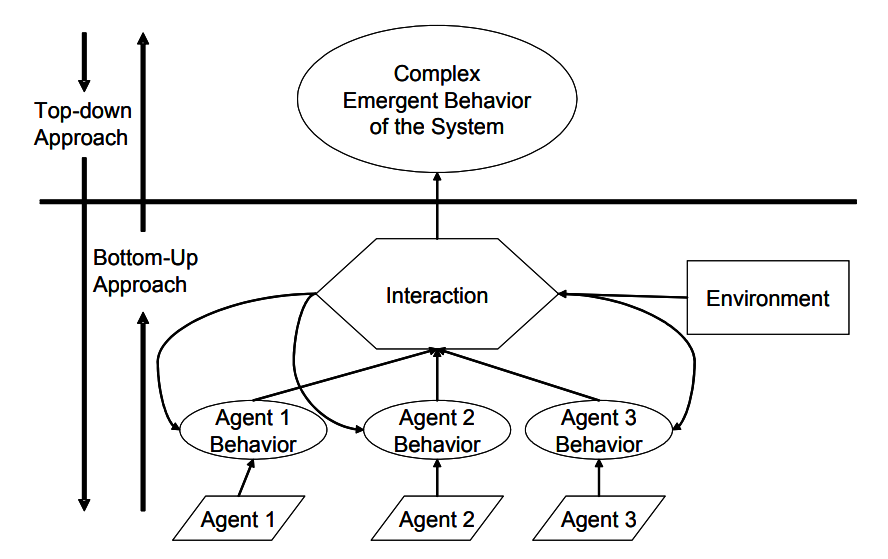
\includegraphics[width=0.8\textwidth]{tex/pics/abm_bottomup.png}
    \caption{Two approaches to model a complex system. Adapted from \textcite{bernhardt2007agent}.}
    \label{abm_bu}
\end{figure}

In general, an ABM is defined by four main elements:
\begin{itemize}
    \item \textbf{The agents}, or computational individuals;
    \item \textbf{The environment}, in which agents are located and move;
    \item \textbf{The time}, and, in particular, the unit of time;
    \item \textbf{The rules}, determining the behaviour of the agents, their interaction and evolution.
\end{itemize}
In agent-based models, a system is described as a collection of autonomous, identifiable entities, called agents, who take decisions and interact between themselves and with the environment in which they are located. Modeling these interactions allows us to capture dynamics and emergent phenomena which otherwise would be unpredictable and impossible to analyze. The interactions are determined both by the rules of the model and by the topology of the environment, which dictates who gets in contact with whom. In fact, just as in real-world, not all agents interact directly with all the other agents all the time, but only with a subset of other agents constituting their \textit{neighborhood}. Typical topologies for ABMs' environment (figure \ref{topologies}) are the ``Cellula Automata" (endowed with either von Neumann ‘4-neighbour’ neighbourhood or Moore's ‘8-neighbour’ neighbourhood), Euclidean spaces, Network structures, the Geographic Information System (GIS) topology, and the 'soup' (where agents' location is irrelevant).  

\begin{figure}
    \centering
    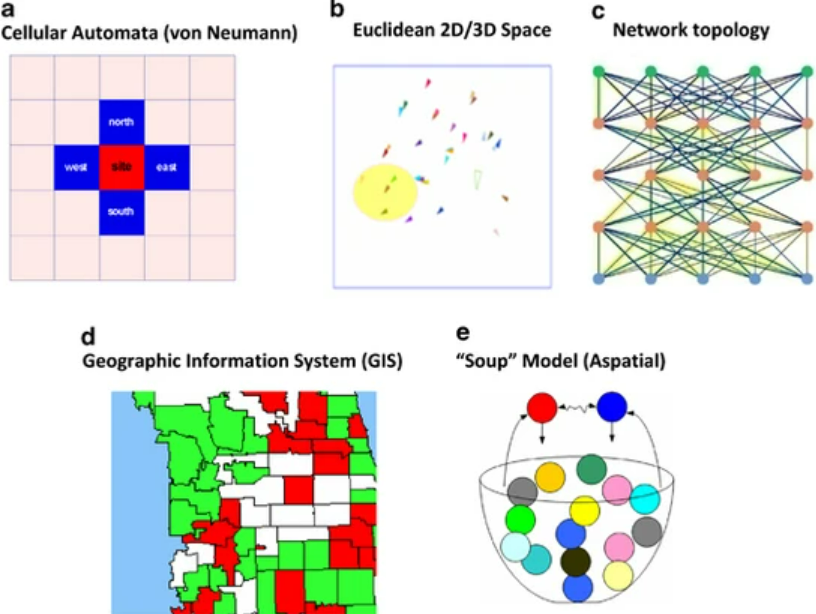
\includegraphics[width=0.7\textwidth]{tex/pics/abm_topologies.png}
    \caption{Common topology structures for ABMs environment. Adapted from \textcite{tutorialABM1}.}
    \label{topologies}
\end{figure}

Agents are characterized by attributes, describing their profile and making them identifiable, and by a state, which varies over time. Attributes allow to potentially define each agent as a different individual exhibiting a different behavior, as to account for real-world heterogeneity. Depending on their state, agents have different admissible actions, which determine their possible behavioral patterns. The individual decision-making process can be modeled with simple, deterministic \textit{if-then} conditional rules, but also with complex probabilistic or mixed rules. Neural networks and genetic algorithms may also be employed, as in \textcite{ALKINANI20228325, abm_rl}, to make the decision-making process more sophisticated and flexible. Usually, agents are ``goal-directed", having goals to achieve and/or objective functions to optimize, and adapting their behavior at future steps on the outcome of previous iterations. Indeed, such kind of model is preferred when it is crucial to have agents that learn and adapt their behavior over time.
Object-oriented programming (OOP) languages are a natural choice to construct agent-based models. Indeed, both agents and environment can be implemented as objects, with their attributes and methods representing the rules of the model. 
  
Agent-based models have recently become increasingly popular, due to their numerous advantages, among which the following should be mentioned:
\begin{itemize}
    \item \textbf{The flexibility}, or the ability to change the degree of description of agents and rules. In particular, one may want to run the simulation with all the agents or a subgroup of agents, or to evolve agents' attributes and rules at any time. This allows to obtain a model with a high level of realism. 
    \item \textbf{The bottom-up approach}, allowing to model the heterogeneity of agents and to describe the system in a more natural way than by specifying a set of equations.
    \item \textbf{Ability to capture emergent phenomena}, arising from the interactions of the individuals under the specified rules, when their collective behavior is much more complex than the sum of each individual behavior. 
\end{itemize}
Although in many fields ABM appear to be the most natural way to represent a system, some weaknesses of this modeling technique should be mentioned. First, ABMs typically require huge amounts of data to be validated, and such data are not always available, especially in the case of systems which have not been extensively studied yet. Moreover, as suggested by \textcite{parunak}, \textit{``the code needed to represent an agent’s behavior in ABM is often longer and more complex than a typical equation in an EBM, and thus potentially more susceptible to representational error"}, which is the error deriving from an inexact representation of the system under study. One last practical issue is that the execution of ABMs simulations can be computationally intensive and time-consuming, an issue that can be at least partly overcome by employing adequate hardware resources and optimizing the code. 

Despite the aforementioned drawbacks, agent-based models have proved to be a versatile technique. The earliest ABM application is thought to be Shelling's model for racial segregation from 1971 \cite{shelling71}, which the author used to demonstrate the spontaneous development of ghettos in social systems. Lately, models of this type have been used in many disciplines, such as physics, biology, but also management sciences, social sciences, economics and ecology. Applications range from models for the immune system \cite{Folcik2007TheBI} to models for existing or hypothetical markets \cite{Charania2006SubOrbitalST, markets2, market3} and for organizational behavior \cite{organization}. Recent applications include models for epidemics and, in particular, COVID-19 pandemic spread \cite{covid1, covid2, covid3}. In the next section, I will focus on applications in the transportation field, which is the main interest of this thesis.


%%%%%%%%%%%%%%%%%%%%%%%%%%%%%%%%%%%%%%%%%%%%%%%%%%%%%%%%%%%%%%%%%%%%%%%

\section{ABM in the transportation field} \label{abm-t}
In the transportation field, agent-based modeling is particularly appropriate to model such systems in which human actions play a critical role. When searching for literature about agent-based models in transportation, a first categorization of the results appears to be evident. There are two main categories in which results can be classified: models for transportation in the context of supply chain and logistics, and models for urban mobility. The two have many points in common, as they both typically imply some vehicle usage and the need to optimize the route such vehicles have to travel, and they often focus on critical situations, like traffic congestion. In general, however, they have different scopes and involve different categories of agents. 

ABMs for logistics attempt to describe the process of freight transport and distribution, which can produce significant economic, social and environmental impacts. In these models, the agents are the main actors in the supply chain that make logistic decisions. In particular, agent based freight models like \cite{log1, log2} identify three main categories of agents: the \textit{suppliers} (goods' producers, wholesalers and shippers who supply the goods), the \textit{receivers} (retailers and end-consumers), and the \textit{transport providers} (freight carriers, couriers or third party logistic service providers taking care of transportation). Some papers use ABMs to control the effects of measures and policies in the transportation sector \cite{log3, log4}; others, instead, aim at solving vehicle routing problems given dynamic decision-making strategies, taking into account external factors, such as road traffic and freight demand \cite{log5}. 

On the other hand, ABMs for urban mobility are used to schematize citizen's behaviour in order to observe population-level dynamics.
\textcite{bernhardt2007agent} identifies four problems related to transportation, and, in particular, related to urban mobility, for which there is an extensive ABM literature: traffic simulation\footnote{There exist several ABM-based simulators for traffic simulation, of which two of the more widely known are TRANSIMS (\url{http://transims.tsasa.lanl.gov/}) and MATSIM (\url{http://www.matsim.org/}).}, pedestrian simulation, lane-changing and travel-demand modeling.  
Agents of ABMs for urban mobility represent the individuals living and moving around in the city, with methods to decide the route to follow and to enable interactions. The real population of the city is often represented, as accurately as possible, by generating a synthetic population, calibrated on sociodemographic information from census data \cite{bib6}. Each agent’s behaviour and movements can be determined through the assignment of a travel diary \cite{bib7}, a sequence of activities the individual makes in a representative day, with details such as departure time, origin and destination. This approach is called \textit{activity-based} \cite{bib8} or \textit{activity-based travel demand model} \cite{bib3} and it has been adopted in several works to study mobility systems of different cities. Its main characteristic is that travel decisions are driven by a collection of activities that form an agenda. The activities are scheduled along with the time, location and means of transport used.
In some cases, also vehicles are modeled as agents of the model, with methods allowing them to move on the network, embark and disembark people. \textcite{Bazghandi_techniques} also adds routes, intersections and signals to the possible categories of agents of the model. 

% LITERATURE OF MODELS SIMILAR TO MINE
The focus of this research is on this second set of models (ABMs for urban mobility) and in particular on cities' public transportation network, to evaluate the efficiency of the public service and the effects of interventions. The idea of using an ABM to study individuals’ mobility patterns is not new in the field of urban science. In \textcite{bib9}, the authors have built an ABM to study the impact of different mobility modes on traffic flow and congestion, with a focus on the city of Cambridge. Another related work is \textcite{bib7}, in which authors have simulated land use and transport demand of an urban area of Sydney. As for Milan, several analyses have been conducted concerning the integration of shared mobility services into the public transport network, the latest ones focusing on how to respond to new needs generated by the pandemic, as in \textcite{bib10}. Still with respect to the pandemic, \textcite{bib11} adopted a simulation approach to evaluate different unlock strategies for public transportation. No significant work has been published yet which considers the flow of passengers as a determinant of the efficiency of Milan’s transport network. The proposed model, presented in details in Chapter \ref{ch:model}, aims at closing this literature gap. 


%%%%%%%%%%%%%%%%%%%%%%%%%%%%%%%%%%%%%%%%%%%%%%%%%%%%%%%%%%%%%%%%%%%

\section{Sensitivity Analysis} \label{sec:ch2_sa}

% 1. What is SA
%   1.1 Definition and why it is useful
%   1.2 Difference from MV and UA
Sensitivity Analysis (SA) is defined as \textit{``the study of how the uncertainty in the output of a model  (numerical or otherwise)  can  be  apportioned to  different  sources  of uncertainty in the model input"} \cite{Saltelli2002SensitivityAF}. 
Given a decision-support model (or, in short, model), \textcite{RAZAVI2021104954} identify several purposes a researcher can address through sensitivity analysis:
\begin{itemize}
    \item Scientific discovery, to explore how the combinations and interactions of hypotheses and parameters affect the system simulated through the model;
    \item Dimensionality reduction, to reduce the complexity of the model;
    \item Data worth assessment, to identify the factors for which one would want to acquire more data;
    \item Decision support, to quantify the sensitivity of an expected outcome to assumptions and constraints.
\end{itemize}

SA differs from Model Validation, which, consists in collecting data both for the input and the output and checking how well the model fits reality. However, according to \textcite{Gass1983FeatureA}, SA is an element of Operational Validity, which is concerned with ensuring that a model is able to produce the expected answers given the inputs, allowing the decision maker to accept or reject it.
Sensitivity Analysis also differs from Uncertainty Analysis (UA) (figure \ref{fig:sensitivity_saltelli}), which ideally should be performed before it, and consists in quantifying the uncertainty in the outputs of the model without attempting to attribute it to any particular input. SA, instead, allows us to decompose the uncertainty that propagates through the model into its sources.

\begin{figure}[H]
    \centering
    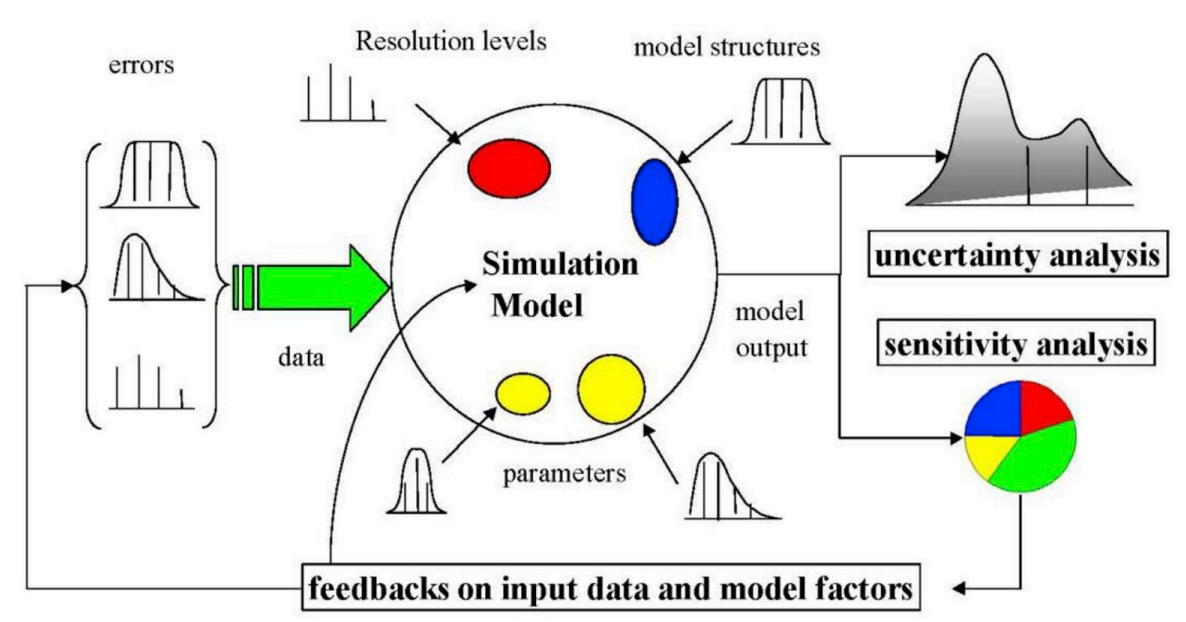
\includegraphics[scale = 0.7]{tex/pics/sensitivity_saltelli.png}
    \caption{Uncertainty and Sensitivity Analysis of a decision model. The grey curve represents the empirical distribution of the output of interest, given that uncertainty propagated from inputs through the model. The pie chart shows the decomposition of uncertainty into its different sources. Adapted from \textcite{saltelli}.}
    \label{fig:sensitivity_saltelli}
\end{figure}

%   1.3 Terminology (model/input/output)
%   1.4 Deterministic vs Stochastic model
When performing Sensitivity Analysis, the decision model is regarded as a map \textit{g} from the input space \textit{X} to the output space \textit{Y}: $g: \mathcal{X} \rightarrow \mathcal{Y}$. Given $n$ model inputs and $D$ outputs, then one can define $X \subseteq \mathbb{R}^n$ and $Y \subseteq \mathbb{R}^D$. Let the vector of model inputs be $\mathbf{x} = (x_1, x_2, ..., x_n)$. It may be the case that not all inputs are the subjects of the sensitivity analysis, so one can construct the index set of inputs $\alpha = (i_1, ..., i_k)$ which are taken into consideration, where $k\leq n$ and the corresponding input vector would be $\textbf{x}_{\alpha} = (x_{i_1}, x_{i_2}, ..., x_{i_k})$. In this setting, one can formalize the difference between a deterministic and a stochastic model. Indeed, a model is said to be deterministic, if by fixing its input \textbf{x} to a value $\textbf{x}^0$, the output remains unchanged \cite{Borgonovo2017SensitivityAA}. Conversely, if a model produces a random value any time it is run with the same fixed input $\textbf{x}^0$, then it is said to be stochastic. In this second case, the analyst would be interested in the conditional distribution of the output given that the input is fixed at $\textbf{x}^0$. Formally speaking, a deterministic model is a particular case of a stochastic model, where the output is a Dirac-$\delta$ function centered at $\textbf{x}_0$. If the model is deterministic, then running the model repeatedly with different inputs and propagating the uncertainty from inputs to outputs is enough to assess the uncertainty in the outputs. 

% 2. The Sensitivity question + SA Settings 
% 3. Deterministic vs Probabilistic frameworks/methods for sensitivity
Before performing sensitivity analysis, a crucial step is to state the goal of the analysis, meaning the insights one is looking for. Formulating the wrong sensitivity question may lead to the use of unsuitable methods and, hence, to obtain wrong or useless insights from the analysis. A first consideration to be made is whether one wants to perform a Local or Global sensitivity analysis. In local sensitivity analysis, one varies the input around a reference value, making finite perturbations. This happens in a deterministic framework, as no probability distribution is assigned to the input. In global sensitivity analysis, instead, the researcher spans the entire input space to assess how interactions of the inputs on the full problem space affect the outputs of the model. If a probability distribution for the inputs is specified, one speaks of probabilistic sensitivity analysis. In this setting, the input vector is a random vector $\textbf{X} = (X_1, ..., X_n)$, whose realizations are $\textbf{x} = (x_1, ..., x_n)$, with cumulative distribution $F_{\textbf{X}}(\textbf{x})$. Uncertainty in the model inputs makes the output $y$ a random variable $Y = g(X)$, of which one could compute statistics. In practice, the modeler runs simulations by generating samples of the inputs, evaluating the model for each sample as to obtain samples of the model outputs through which are obtained the empirical cumulative distribution functions of the outputs.

To formalize the choice of the sensitivity question, researchers have developed the concept of sensitivity analysis settings \cite{Saltelli2002SensitivityAF, Saltelli2002OnTR}, representing the goals of sensitivity analysis, but also the main corresponding methods used to achieve them. \textcite{Borgonovo2016SensitivityAA}, in their literature review, define a setting as \textit{``a formulation of the sensitivity analysis quest which is stated before the sensitivity analysis is carried out"}, and identify five main settings:
\begin{itemize} \label{sa_settings}
    \item \textbf{Factor prioritization}: the goal is to identify the main drivers of output changes, according to some importance measure, and to be able to focus the efforts of data collection on the acquisition of data related to the most important inputs as to reduce uncertainty in the results. Appropriate methods are finite differences (with total effects visualized through \textit{Tornado diagrams}) in deterministic frameworks, or differentiation-based measures in probabilistic analysis.
    \item \textbf{Factor fixing}: here the goal is similar but opposite to that of factor prioritization: identifying the least influential parameters, which can then be fixed as to reduce complexity of the model and save computational cost.
    \item \textbf{Direction of change}: in this case, one is interested to know whether an increase (or a decrease) in a model input provokes an increase (or a decrease) in model outputs. For example, one may want to look at the sign of finite change sensitivity indices or of partial derivatives, in the deterministic and probabilistic framework respectively.
    \item \textbf{Interaction quantification}: the goal is to analyze the structure of the model to understand whether there are interactions among the model inputs. Usually, researchers focus on two-elements interactions, since higher-level interactions are computationally expensive to analyze.
    \item \textbf{Robustness (or Stability)}: decision-makers are interested in determining whether variation to parameters' reference value invalidate the conclusions of the analysis and assessing the region of the model input space over which, instead, there is no change.
\end{itemize}



%%%%%%%%%%%%%%%%%%%%%%%%%%%%%%%%%%%%%%%%%%%%%%%%%%%%%%%%%%%%%%%%%%

\section{Sensitivity Analysis of ABMs} \label{sa-abm}


% 1. perchè fare sa degli abm
% 2. challenges?
%     - two levels (micro vs macro)
%     - stochastic --> min simulation runs
%     - spatio-temporal outcome
% 3. methods
% 4. borgo steps

In order for an ABM to be useful to learn about a complex system, it is essential to compare the effects on output measures under different parameters configurations. Sensitivity analysis allows examining the robustness of the model to parameter changes, to ensure that the conclusions one takes do not depend on specific sets of assumptions. Analyzing the behavior of the model becomes even more crucial if the researcher is interested in capturing, through the model, early signals of the system being in a critical condition. Indeed, SA helps to identify the hidden model dynamics, by inspecting the effects of parameter changes into model output. Moreover, it plays an important role in recognizing if there are computationally expensive assumptions of the model that can be replaced with cheaper ones without compromising the results.  

There are, however, several structural properties of ABMs that make the application of statistical methods to perform sensitivity or uncertainty analysis quite challenging in this framework. First, agent-based models have at least two levels of detail: a \textit{micro-level}, consisting of everything concerning agents and their individual behavior, and a \textit{macro-level}, comprising the environment and the emerging macroscopic patterns. This duality is also reflected in the results of ABM simulations, as one typically obtains both individual-level and system-level outputs, gaining distinct managerial insights. Moreover, interactions between agents are typically non-linear and may change over time, due to agents' learning and emergent dynamics. With non-linear individual interactions, there might be also non-linear input-output relations, which may be difficult to capture adopting standard sensitivity methods. As a consequence, similar parameters may lead to totally different outputs, while completely different settings could produce similar system behaviors. Furthermore, from an ABM one is able to obtain outputs with spatio-temporal dimension, which are really complex and may exhibit the effect of several dynamics. Hence, careful analysis is required to decompose the different elements, adopting appropriate techniques for time series (e.g. moving averages, exponential smoothing or autoregressive modeling to decompose trend, cycle, seasonality and randomness) and suitable visualization tools for spatial analysis. Finally, to evaluate stochastic ABMs, one needs to compute statistics across multiple model runs in order to average out the random component. It is crucial to compute in advance the minimum number of runs required in order to secure stability of the outcome's variance. \textcite{Lee2015TheCO} review several methods to overcome the aforementioned challenges. 

To gain insights about the hidden dynamics of the model, \textcite{Broeke2016WhichSA} suggest starting any sensitivity analysis of ABM with One-factor-at-a-time (OFAT) analysis, meaning evaluating the model at different values for one parameter, while keeping all others' values fixed. \\ Through the OFAT experimental design, one is able to compute the so-called \textit{main effects} of the model inputs, that can later be visualized through Tornado diagrams and their normalized version, or \textit{Newton quotients}. Varying more inputs at the same time, one is able to perform a complete finite-difference analysis, that is, to compute also \textit{interaction effects} and the \textit{total finite change effect} of each parameter. \\ Local sensitivity analysis is performed in case one evaluates only a finite set of points into the input space. If parameters are discrete, then for a global sensitivity analysis it is enough to consider a \textit{full factorial} design, that is, to evaluate all possible combinations of input values. Computationally cheaper solutions, as the \textit{fractional factorial} design, have been proposed, allowing to compute the interaction effect up to a certain order. Standard techniques for global sensitivity analysis are, instead, variance-based, distribution-based or regression-based methods, which, however, \textcite{Broeke2016WhichSA} argue that do not always address the previously stated issues of agent-based modeling. \\ A further issue is that most applications of sensitivity analysis of agent-based models only tackle variations in input parameters, while forgetting to conduct an analysis of the effects of changing ``non-parametric" elements of the model. \textcite{Borgonovo2022SensitivityAO} stress that \textit{``a researcher who is performing a sensitivity analysis involving only parameters is implicitly fixing a substantial portion of an agent-based simulation"}. Thus, they propose an approach to conduct the sensitivity analysis of ABMs allowing to treat also the variation of non-parametric elements and behavioral rules, and to quantify the interaction of parameters and procedures, in a way that is defined \textit{``in between a local and a global approach"}. \\ The proposed protocol consists of the following six steps (as in figure \ref{fig:borgonovo_protocol}):

\begin{figure}[t!]
    \centering
    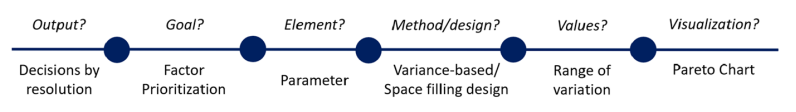
\includegraphics[width = \textwidth]{tex/pics/borgonovo_protocol.png}
    \caption{The six steps for sensitivity analysis of ABMs, adapted from \textcite{Borgonovo2022SensitivityAO}.}
    \label{fig:borgonovo_protocol}
\end{figure}

\begin{enumerate}
    \item \textbf{Choosing the output (or the outputs) of interest.} Depending on whether the model is deterministic or stochastic, the quantity of interest could be the output of the model itself or, if that is a distribution, one of its summary statistics. 
    \item \textbf{Deciding the goal of the sensitivity analysis to pursue (i.e. setting).} The researcher may want to increase their understanding of the model dynamics or to produce insights for the decision-makers. Possible settings have been described above in Section \ref{sa_settings}.
    \item \textbf{Selecting the elements of the model to vary, among parameters and procedures.} The authors propose a conceptual structure for ABMs (graphically represented in \ref{fig:borgonovo_elements}) to classify the ``moving parts" of the model that can be subject to sensitivity analysis, among which the researcher is called to pick those they're interested in varying. In particular, the structure distinguishes between two distinct subsets of assumptions, \textit{Parameters} (C) and \textit{Procedures} (E). Parameters are cardinal quantities, characterizing either the agents, the environment or some properties of the simulation; they are determined in advance, before running the simulations, and influence the evolution of the model. On the other hand, procedures are non-cardinal and represent rules of the model or of the simulation; for instance, they could regulate the initialization of parameters or define agents' behavior. The authors propose to \textit{``treat the alternative specifications of a non-parametric element as the levels of a categorical variable"} and to conduct the sensitivity analysis by considering a full factorial design. 
    \item \textbf{Choosing the most appropriate methods to perform the sensitivity analysis for the goal-element-model combination.} Once the goal and the elements of interest have been defined, one has to decide the scale of the analysis (local or global) and, consequently, the methods to adopt. 
    \item \textbf{Assigning numerical values to the parameters of the model.} If the scale of the analysis is local, then the researcher defines the values of the base case and those of one or more alternative scenarios. In case of a global probabilistic analysis, instead, the analyst specifies the support and the distributions of each input of interest.
    \item \textbf{Selecting the appropriate visualization tools to present the results of the analysis.} Choosing the wrong visualization tool may result in a non-effective communication of the results to the stakeholders that have to make decisions out of the simulation's conclusions. Special care must be taken in case of stochastic ABMs, from which one obtains results in the form of distributions. To deal with changes in statistics of those distributions, in fact, it may be required to conduct statistical significance tests.
\end{enumerate}

Later, in Chapter \ref{ch:sa}, I will adopt this protocol to perform the sensitivity analysis of an agent-based model for the simulation of traffic flows on Milan's public transportation system, described in detail in Chapter \ref{ch:model}.
\begin{figure}[H]
    \centering
    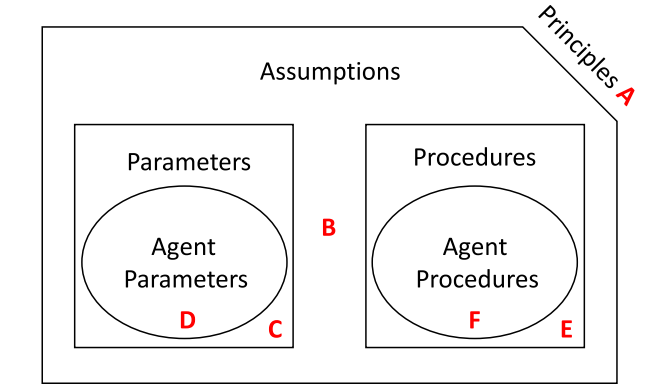
\includegraphics[width = 0.9\textwidth]{tex/pics/borgonovo_elements.png}
    \caption{The four types of elements of an agent-based model, as per \textcite{Borgonovo2022SensitivityAO}: principles, assumptions, parameters and procedures.}
    \label{fig:borgonovo_elements}
\end{figure}